\section{Duodécima iteración de la Fase 5: Cambio en el manejo de las pestañas}
\label{sec:F5I12}

Antes de seguir, otra pausa para mejorar el manejo. Tras poner la pestaña de cartucho, no era lógico tenerla como la última pestaña, cuando el proceso necesario es cargar el setup y luego cargar el cartucho.

Para ello cambio el sistema para poner las pestañas en el orden adecuado y, de paso, añado la posibilidad de crear el fichero de setup desde la propia aplicación, de manera que se pueda partir de cero sin escribir ningún \emph{json} a mano.

\subsection{Nueva pestaña y nuevo orden}
\label{sec:F5I12Orden}

La idea inicial fue poner en la pestaña Cartucho los datos separados en dos grupos, GWS y GWB, pero he visto mejor dividirlo en dos pestañas: añadir una nueva pestaña para los datos del setup y dejar en la del cartucho solo los propios de este.

Esto me lleva a reordenar las pestañas en un orden más natural, de forma que aparezcan en el orden adecuado si creamos todo desde cero. Es más lógico, y además permite visualizar que, cuando un dato cambia en una pestaña, afecta a todas las posteriores, y eso se ve de forma visual por el nuevo orden:\\

\centerline{\textbf{Setup - Cartucho - Editor - Sprites - Simulador}}

\vspace{0.5em}

Las pestañas no estarán activas si faltan los datos necesarios para su manejo, de forma que quede claro el orden adecuado:

\begin{table}[H]
	\centering
	\begin{tabular}{|l|p{9cm}|}
		\hline
		\textbf{Pestaña} & \textbf{Se activa} \\ \hline
		Setup & Siempre. \\ \hline
		Cartucho & Hay un setup aplicado. \\ \hline
		Editor & Hay un cartucho aplicado (GWB o GWI). \\ \hline
		Sprites & Está activa \emph{Editor}. \\ \hline
		Simulador & Hay datos de segmentos o un GWI/GWB cargado. \\ \hline
	\end{tabular}
	\caption{Cuándo está activa cada pestaña.}
\end{table}

Al arrancar solo está activada la pestaña \textbf{Setup}, se van activando conforme se cargan datos, pero durante una partida la única activa es la del simulador.

\begin{figure}[H]
	\centering
	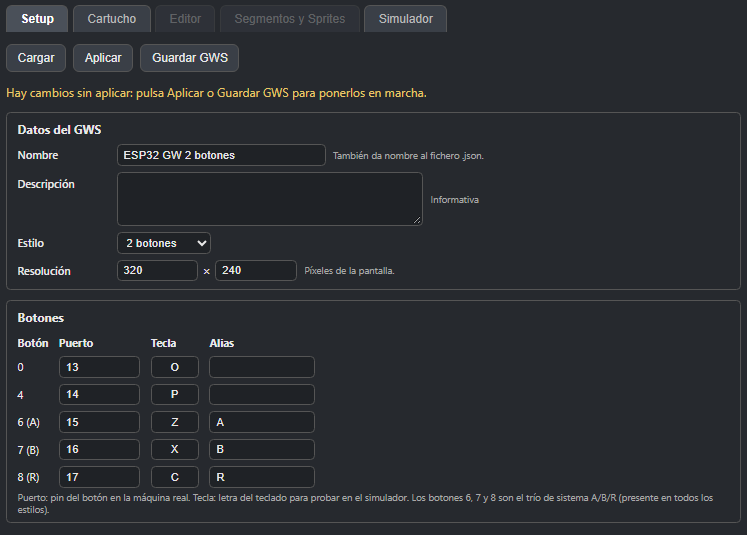
\includegraphics[width=0.60\linewidth]{imagenes/Propias/C05-I027}
	\caption[Pestaña de setup]{Pestaña de Setup}
	\label{fig:c05-i027}
\end{figure}

\subsection{Cambios en los botones}
\label{sec:F5I12Botones}

Para mejorar más el manejo, cambio de lugar los botones, ubicándolos dentro de cada pestaña. Así se ve más claro lo que se puede manejar en cada una. Desaparece la barra de botones superior; solo se mantiene siempre visible la línea de estado.

\begin{itemize}
	\item \textbf{Setup}: botones para \textbf{Cargar}, \textbf{Aplicar} y \textbf{Guardar GWS} (que guarda y aplica). No hay más pestañas activas hasta que se aplica o guarda, momento en que se activa la siguiente. Si se cambia algo no se hace nada hasta que se pulse Aplicar o Guardar, que limpia todo lo que depende del setup (cartucho, segmentos, sprites\ldots), como hace ahora el cargar un setup nuevo.
	
	\item \textbf{Cartucho}: botones para \textbf{Cargar GWB} (carpeta), \textbf{Cargar GWB} (ZIP), \textbf{Cargar GWI}, \textbf{Aplicar} y \textbf{Guardar GWB}. Al aplicar se activan las demás pestañas. Aplicar un cambio, y en particular en la imagen de segmentos, elimina los datos de las pestañas del Editor y de Sprites, como si hubiésemos cargado un nuevo setup y luego el GWB. Esto es importante para los sprites, que se extraen de esa imagen.
	
	\item \textbf{Editor}: botones para \textbf{Cargar GWB} (carpeta y ZIP), \textbf{Cargar GWI}, \textbf{Deshacer}, \textbf{Rehacer}, \textbf{Verificar y Guardar} y \textbf{Generar GWB+GWI+GWC}, que genera también el GWB (iteración~\ref{sec:F5I10}) para que los tres vayan de la mano.
	
	\item \textbf{Sprites}: ningún botón en su interior, es una pestaña meramente informativa.
	
	\item \textbf{Simulador}: botones para \textbf{Cargar GWI} y \textbf{Cargar GWC}, lo necesario para ejecutar.
\end{itemize}

El código que habilita o deshabilita los botones y que atiende sus pulsaciones es el mismo que ya existía: solo cambia el lugar donde se muestran. Pero un mismo botón puede aparecer en varias pestañas (Cargar GWI está en tres), y un identificador HTML no puede repetirse, por lo que cada pestaña tiene su propio elemento con su identificador y todos comparten el mismo manejador, y la misma lista de botones se habilita o deshabilita conjuntamente.

\subsection{Datos pendientes de aplicar}
\label{sec:F5I12Aplicar}

Las dos fichas (Setup y Cartucho) funcionan ahora como un \textbf{borrador}: lo que se escribe o se carga en ellas no afecta al resto del programa hasta que se pulsa Aplicar (o Guardar que hace un aplicar implícito). Esto evita perder un cartucho en edición por un clic.

\begin{itemize}
	\item \textbf{Cargar un fichero} (GWS, GWB o GWI) rellena la ficha y la aplica directamente, como hoy.
	\item \textbf{Aplicar} toma lo que hay en la ficha y lo pone en marcha con el mismo flujo que una carga de fichero, sin pasar por él: en el Setup, valida y aplica la máquina; en el Cartucho, construye el cartucho desde la ficha, lo valida y lo entrega al editor (extracción de sprites, mapa y botonera), de modo que un cartucho creado en la ficha y uno cargado de disco son indistinguibles para el resto del programa. Esto cumple la entrega directa de la ficha al editor que quedó como mejora futura en la iteración~\ref{sec:F5I10}.
	\item \textbf{Efecto en cascada:} aplicar un setup elimina el cartucho y todo lo que de él depende; aplicar un cartucho elimina los datos del Editor y de Sprites. Se hace siempre, aunque solo haya cambiado un dato menor: es más simple y evita mezclas erróneas.
	\item \textbf{Indicación visual:} cada ficha avisa de que tiene cambios sin aplicar, para que no se confunda lo que se ve con lo que está en marcha.
	\item \textbf{Generar y guardar desde el Editor} usan siempre los datos \emph{aplicados}, no los del borrador, de forma que el GWI y el GWC sean coherentes con los segmentos que realmente hay en memoria.
\end{itemize}

Este cambio sustituye el bloqueo de la imagen img\_s con segmentos en memoria de la iteración~\ref{sec:F5I10}: ya no hace falta bloquear los botones de esa imagen, pues cambiarla solo tiene efecto al pulsar Aplicar, y entonces se descartan los segmentos y se extraen de nuevo.

\subsection{La ficha de Setup}
\label{sec:F5I12Ficha}

La nueva pestaña muestra la ficha con los datos del setup, que permite crear y manipular los ficheros de setup (GWS), con estos datos:

\begin{itemize}
	\item \textbf{nombre}: el que se desea dar al setup; sirve también para dar nombre al fichero GWS que se genera (sin caracteres no válidos en un nombre de fichero).
	
	\item \textbf{descripcion}: pequeña descripción de la máquina y de su manejo. Es un campo \textbf{nuevo} del GWS, opcional, y solo informativo.
	
	\item \textbf{estilo}: el de los botones (2, 4, 5). 
	
	\item \textbf{resolucion}: ancho y alto de la pantalla.
	
	\item Los botones: tabla con los botones posibles según el estilo, incluido siempre el trío del sistema A/B/R (6, 7 y 8), con su definición para el sistema externo: 
	\begin{itemize}
		\item \textbf{puerto}: qué pin del aparato se usa para manejar el botón. 
		\item \textbf{tecla}: la del teclado del PC con que se prueba en el simulador
		\item \textbf{alias}: Alias posible de la tecla, se puede usar en lugar del número.	
	\end{itemize}
\end{itemize}

La verificación del GWS reutiliza la validación que ya aplica \emph{baseDirector} al cargar un setup, con los mismos errores bloqueantes (estilo y botones coherentes, puertos y teclas sin repetir, resolución válida), de modo que un GWS creado en la ficha se puede cargar siempre. Los hallazgos se muestran en la propia ficha, como en la del cartucho.

Al cargar un GWS la ficha se rellena con todos sus datos, incluidos puertos y teclas. Para ello, la ficha del setup es un módulo independiente, igual que la del cartucho, que no conoce al director: el director la rellena y la consulta.

\subsection{Cambios en otras partes del código}
\label{sec:F5I12Codigo}

\begin{itemize}
	\item \textbf{index.html y estilos:} se mueven los botones a sus pestañas, y se eliminan las reglas de CSS que los ocultaban según la pestaña activa. Se reordenan las pestañas y se añade la nueva.
	\item \textbf{Módulo de la ficha de Setup (nuevo):} campos, tabla de botones, verificación y guardado del GWS.
	\item \textbf{baseDirector.js:} nuevo orden y reglas de habilitación de las pestañas; separación de la carga del setup en leer y aplicar, para poder aplicar desde la ficha; función equivalente para el cartucho (aplicar un cartucho ya leído, que sirve tanto a la carga de fichero como a la ficha).
	\item \textbf{baseFicha.js:} el botón Aplicar y el aviso de cambios sin aplicar; la ficha deja de bloquear img\_s.
\end{itemize}

\subsection{Qué cambia para el usuario}
\label{sec:F5I12Usuario}

El orden de las pestañas refleja el del trabajo, nada se puede hacer sin los datos previos, cada pestaña tiene sus botones a la vista y es posible partir de cero: crear el setup, crear el cartucho y generar los ficheros sin escribir ningún \emph{json}.

\subsection{Pruebas de la iteración}
\label{sec:F5I12Pruebas}

\begin{itemize}
	\item Al arrancar solo está activa la pestaña Setup; tras aplicar un setup se activan Cartucho y Simulador, y tras aplicar un cartucho, Editor y Sprites.
	\item Con un GWC cargado, Editor y Sprites quedan deshabilitadas; durante una partida solo está activo el Simulador.
	\item Cada botón está en la pestaña indicada, y los repetidos (Cargar GWI) funcionan igual en todas.
	\item Cargar un GWS rellena la ficha, incluidos puertos y teclas; guardarlo y volverlo a cargar produce la misma ficha.
	\item Un GWS creado desde cero, aplicado, permite cargar un cartucho; los errores de validación (puertos o teclas repetidos, estilo incoherente) bloquean el guardado.
	\item Cambiar algo en la ficha sin pulsar Aplicar no altera el simulador ni el editor, y se avisa de los cambios sin aplicar.
	\item Aplicar un setup nuevo elimina el cartucho y sus datos; aplicar un cartucho con otra img\_s elimina y recalcula segmentos y sprites.
	\item Un cartucho creado en la ficha, aplicado, es indistinguible de uno cargado: se edita, genera y juega igual.
	\item Generar usa los datos aplicados aunque la ficha tenga cambios sin aplicar.
\end{itemize}

\subsection{Mejoras pendientes}
\label{sec:F5I12Pendientes}

\begin{itemize}
	\item Poder editar el setup en caliente, aplicando los cambios sin perder el cartucho cuando no le afecten.
	\item Un solo panel de carga de ficheros que reconozca cualquier tipo por su contenido (\ref{sec:F5I9}), con lo que desaparecerían los botones de carga duplicados.
	\item Usar el campo \texttt{descripcion} del GWS, por ejemplo en el selector de máquinas.
\end{itemize}